% Preamble
\documentclass{ctexart}

% Packages
\usepackage{amsmath}

\title{唯一回文子串问题数据结构的改进}
\author{申治洺}
\date{2024年5月20日}

% Document
\begin{document}

    \section{本篇论文概述}\label{sec:1}
    
本文在概述原文时,着重介绍数据结构的设计。对于原文中涉及的大量引理(Lemma)、定理(Theorem)、命题(Proposition)、
推论(Corollary),本文直接引用其中的结论,不再关注其证明过程,因为原文提供了详尽的证明或证明所在的参考文献。
由于原文中直接引用了一些不太常用的数据结构,如后缀树、van Emde Boas树等,本文会适当补充相关数据结构的定义、实现、性质。
对于原文中定义不够明确的概念,本文给出了严格的定义,并描述和论证了相关性质。

\subsection{问题引入}\label{subsec:intro}

\begin{description}
    \item [MUPS] 给定串$T$,$1 \leq i \leq j \leq ||T||$,回文子串$u = T[i..j]$,如果$u$在$T$中是唯一的,
    $u^{\prime} = T[i + 1..j - 1]$在$T$中不唯一,则称$u$是$T$的极小唯一回文子串(minimal unique palindromic substring).
    \item [interval SUPS] 给定串$T$和区间$[p,q]$,回文子串$v = T[i..j]$,$v$在$T$中唯一且包含区间$[p,q]$,
    任何更短的包含区间$[p,q]$的$T$的回文子串都在$T$中不唯一,则称$v$是对区间$[p,q]$的$T$的最短唯一回文子串
    (shortest unique palindromic substring),记作$v = \mathrm{SUPS}_T ([p,q])$.
    \item[point SUPS] 区间SUPS问题在$p = q$的情况下退化为点的SUPS问题,记作$v = \mathrm{SUPS}_T (p)$.
    \item[ME] MUPS向外扩展,即每次起点向前移动一位,终点向后移动一位,直至破坏回文性为止。
    在此过程中可以得到“极小唯一回文子串的极大扩展”(maximal extension of MUPS).
    \item[MP] 对任意一个半整数,即1, 1.5, 2, 2.5 .. , n \footnote{原文中串从1开始标号,本文也采用这种规范。},
    都能求得以其为中心的极大回文子串(maximal palindrome).
\end{description}

需要注意的是,MUPS是极小的,强调的是MUPS都无法在自身基础上再缩小一点,因为再缩小会违背MUPS的唯一性,
MUPS的定义并不关心每个MUPS与其他MUPS的长度比较。SUPS是最短的,SUPS的定义基于多个包含给定区间或点的回文子串的长度比较,
但这并不意味着SUPS仅有1个。原文中的Theorem 1说明SUPS至多只有4个。

由MUPS的定义可知,MUPS具有唯一性,此外MUPS不存在嵌套的情况,可用反证法论证如下:

取MUPS $M_1 = T[s_1..e_1]$,MUPS $M_2 = [s_2..e_2]$,满足$s_1 \leq s_2 \leq e_1 \leq e_2 $,
且$s_1 \leq s_2$和$e_1 \leq e_2$不能同时取等。找到$M_1$的对称轴$l$,若$M_2$关于$l$对称,则$M_1$显然不满足MUPS定义中的极小性;
若$M_2$不关于$l$对称,则取串$M_3$关于轴$l$与$M_2$对称,由于$M_2$是回文串,$M_3$与$M_2$完全一致,显然违背了$M_2$作为MUPS的唯一性。

原文中使用的“极大回文子串”(maximal palindrome)一词,其实兼指ME和MP。这里明确地区分了这两个概念,并在下文探讨两者的性质和联系。

ME具有唯一性和非嵌套性,可用反证法论证如下:

假设存在两个完全一致的ME$m_1$和$m_2$,$m_1$对应的MUPS为$M_1$,以$m_1$和$M_1$的相对位置关系在$m_2$中找到回文子串$M_2$,
$M_2$一定与$M_1$不重合,于是违背了$M_1$作为SUPS的唯一性。ME的唯一性得证。

取ME$m_1 = T[s_1..e_1]$,ME$m_2 = [s_2..e_2]$,满足$s_1 \leq s_2 \leq e_1 \leq e_2 $,
且$s_1 \leq s_2$和$e_1 \leq e_2$不能同时取等。找到$m_1$的对称轴$l$,若$m_2$关于$l$对称,则$m_2$不满足ME定义中的极大性;
若$m_2$不关于$l$对称,则取串$m_3$关于轴$l$与$m_2$对称,由于$m_2$是回文串,$m_3$与$m_2$完全一致,
$m_2$不满足上文已证的ME的唯一性。ME的非嵌套性得证。

显然,MP完全包含了ME。通常情况下,MP包含了大量的空串和单字符串,并有大量重复情况。例如,串$T = \mathrm{babbbabbababb}$,
以2为中心的MP $\mathrm{bab}$和以11为中心的MP $\mathrm{bab}$发生重复,因此两者都不包含在ME中。

事实上,唯一且非空的MP等同于ME。证明如下:

对任意非空的MP,定义“缩小串集”为MP缩小\footnote{类似于扩展,缩小指每次将回文串的起点向后移动一位,终点向前移动一位。}过程中产生的所有回文串的总和。
易知,“缩小串集”包含了所有回文子串,也就包含了所有ME。不唯一的MP缩小产生的回文串也是不唯一的,因而不能产生ME。对唯一的MP进行缩小,缩小的尽头是空串,
必然丧失唯一性。因此,在缩小的过程中一定存在唯一性发生改变的临界,即可找到一个MUPS,则该唯一的MP也就成为一个ME。综上,唯一且非空的MP与ME一一对应。

\subsubsection{最长公共扩展(LCE)与后缀树(Suffix tree)}\label{subsubsec:lce}

对于长度为$n$的串$S$,后缀树(Suffix tree)定义为这样一棵树,满足如下五个条件\cite{suffix}:
\begin{itemize}
    \item 有$n$个子节点,分别编号$1$至$n$
    \item 除根节点外,每个非叶节点都有至少两个子节点
    \item 每条边都用$S$的一个非空子串来标记
    \item 起始于同一节点的两条边不能有同一字符开头的标记
    \item 从根节点到叶节点$i$,将所有边的标记依次拼接起来,可得到后缀$S[i..n]$
\end{itemize}

\begin{figure*}[h]
    \centering
    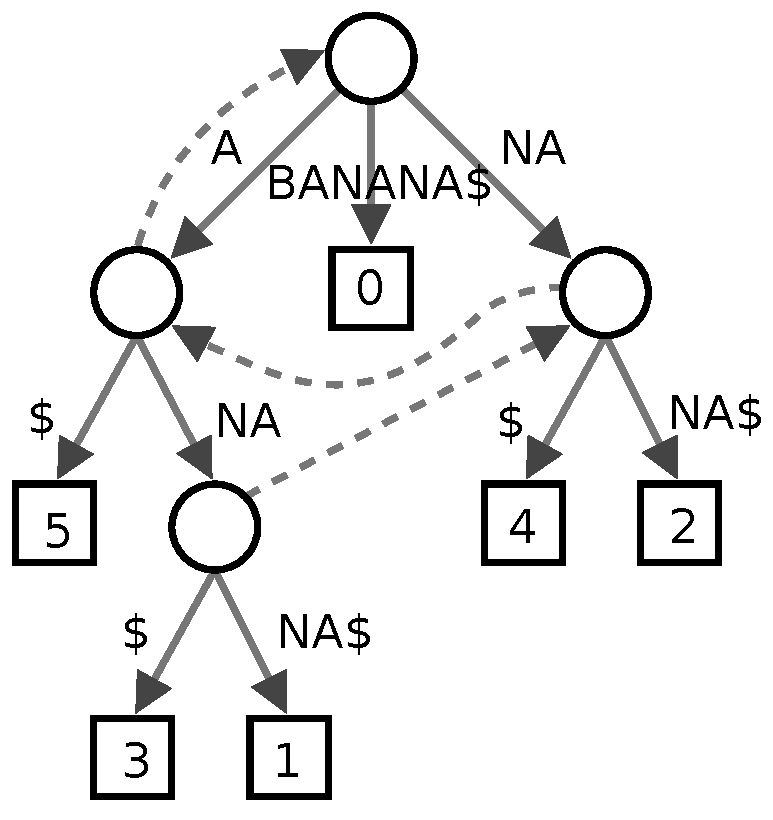
\includegraphics[width=0.8\textwidth]{resources/fig/Suffix_tree_BANANA}
    \caption{$\mathrm{BANANA\$}$的后缀树,虚线为构建过程中的辅助线\cite{suffix}}
\end{figure*}

最长公共扩展(longest common extension, LCE)问题是对一个给定的串$T$,给定的整数$i,j$,满足$1 \leq i,j \leq n$,
计算出两个后缀$T[i..n]$和$T[j..n]$的最长公共前缀的长度。

\subsubsection{区域最小值请求(RmQ)及变体LogRmQ}\label{subsubsec:rmq}

区域最小值请求(range minimum query ,RmQ)是对一个给定的整型数组$A$,$A$上的两个下标$i,j$,满足$i \leq j$,
计算出下标$k$使得$A[k]$为$A[i..j]$上的最小值。注意RmQ数据结构并不要求整型数组有序。

\subsection{前驱(Predecessor)、后继(Successor)与van Emde Boas树}\label{subsec:van}

对一个不减的整型数组$B$,给定整型数$x$,定义前驱(Predecessor)是小于$x$的最大值;同理,定义后继(Successor)是大于$x$的最小值。

\subsection{Inoue算法概述}\label{subsec:inoue}

\subsection{原文对Inoue算法的改进}\label{subsec:progress}

\subsection{原文算法的示例}\label{subsec:example}


    \section{相关领域综述}\label{sec:2}
    
回文串是从前向后和从后向前读取结果相同的序列。由于其独特的性质以及在模式识别、数据压缩和DNA序列分析中的广泛应用,在生物信息学、计算机科学等领域,
对回文串的研究不断。本节探讨了回文串的主要研究方向,包括但不限于极小唯一回文子串、最短唯一回文子串和极大回文子串。

\subsection{极小唯一回文子串}\label{subsec:mups}

极小唯一回文子串(MUPS)的定义和性质详见\ref{subsec:intro}。求解MUPS的算法设计策略总结如下:
\begin{itemize}
    \item 基于后缀树。对输入的串构建后缀树,从后缀树中获取所有极小唯一的子串,再从中提取回文串\cite{Gusfield_1997}。
    这种策略需要消耗$O(n)$的时间以完成构建后缀树的预处理\cite{Ukkonen95}。
    \item 基于动态规划。使用一个动态规划的表格标记出所有回文子串,再依次检查每个回文子串是否唯一。时间复杂度为$O(n)$\cite{Manacher75}。
\end{itemize}

\subsection{极大回文子串}\label{subsec:mp}

极大回文子串(MP)的定义和性质详见\ref{subsec:intro}。求解MP的算法设计策略总结如下:
\begin{itemize}
    \item 使用Manacher算法\cite{Manacher75}。这是一个求解MP的在线(on-line)算法\footnote{即支持一位一位地按顺序输入串,运行过程中的结果是对于已输入串的问题解。},可以在线性时间内获得结果。
    \item 使用Eertree (Palindromic Tree)\cite{RubinchikS18}。这种数据结构可以储存所有互异回文子串,以便快速求解MP。
\end{itemize}

\subsection{最短唯一回文子串}\label{subsec:sups}

最短唯一回文子串(SUPS)的定义和性质详见\ref{subsec:intro}。求解SUPS问题,可以使用Inoue算法\cite{Inoue2018},详见\ref{subsec:inoue};
以及原文\cite{Mieno2024}对Inoue算法的改进算法,详见\ref{subsec:progress}和\ref{subsec:example}。

\subsection{回文分解}\label{subsec:factorize}
回文分解(palindromic factorization)是将一个串划分为最少数量的回文串的过程,常用于数据压缩和文本挖掘。借助Eertree数据结构,
k-分解问题可以在$O(kn)$时间内完成\cite{RubinchikS18}。


    \section{当前算法的不足}\label{sec:3}
    
本节从最短唯一回文子串、极小唯一回文子串、极大回文子串这三个方面介绍回文串领域的主要研究成果。


    \section{改进算法的提出}\label{sec:4}
    
本节为\ref{sec:3}提出的全动态模型设计实现算法。原文6.2节已实现支持任一位的替换的半动态模型,所以这里只需实现任一位的删除和添加操作的情形。

\subsection{删除情形}\label{subsec:del}

由于计算MUPS集合\cite{Manacher75}和LCE\cite{Ukkonen95}的算法都是在线的。可以对内部细微数据结构(如后缀树中的节点和边)进行标记,
从而可以在后面的任意时刻退回到刚读入第$i$位时的状态$S_i$.设外部请求删除第$k$位,则立刻让MUPS集合和LCE退回状态$S_{k-1}$.
又由\cite{Mieno2022}知每次在串尾插入一位,改变的MUPS的数量为常数,且可以在均摊的$O(\log\sigma)$时间内检测到变化并调整MUPS集合。
从原来的第$k+1$位开始重新插入,共经$m = n - k$次插入,若忽略对数因子,则可以在$\tilde{O}(m)$时间内完成对数据结构的调整。

\subsection{添加情形}\label{subsec:add}

仿照\ref{subsec:del},设外部请求在第$k$位和第$k+1$位的间隔处添加一位,则立刻让MUPS集合和LCE退回状态$S_{k}$.
插入新位,再从原来的第$k+1$位开始重新插入,共经$m = n - k$次插入,若忽略对数因子,则可以在$\tilde{O}(m)$时间内完成对数据结构的调整。

\subsection{回顾与展望}\label{subsec:future}

本节实现的$\tilde{O}(m)$时间复杂度的算法适用于被操作为靠近串尾的情况,如果不满足该条件,则实际的时间复杂度与$O(n)$并无太大差别。
而实际上,每次重新计算MUPS集合、MP集合或LCE也只需要$O(n)$的时间。原文中能设计出比$O(n)$高效的算法,得益于论文\cite{Mieno2022,Mieno2021}
提出了特定情形下修改MUPS集合的高效算法,而这两篇论文中的算法都基于Eertree\cite{RubinchikS18}数据结构。
未来实现高效的全动态模型SUPS算法可能还是要从Eertree着手。


    \bibliographystyle{plain}
    \bibliography{resources/references}
\end{document}